\documentclass{article}
\usepackage[utf8]{inputenc}
\usepackage[margin = 0.8in]{geometry}
\usepackage{graphicx}
\usepackage{amsmath, amssymb}
\usepackage{subcaption}
\usepackage{multirow}
\usepackage{float}
\usepackage{listings}


\title{RBE502 - Homework Set 2}
\author{Keith Chester}
\date{Due date: September 8, 2021}

\begin{document}
\maketitle

\section*{Problem 1}
We are presented with two figures representing two figures, seen below:

\begin{figure}[H]
    \centering
    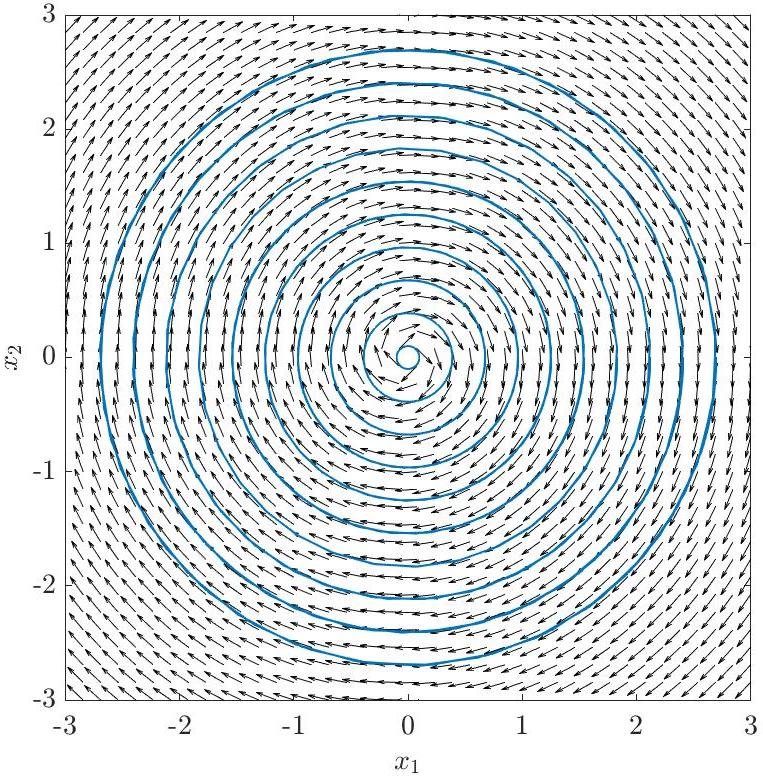
\includegraphics[width = 0.4\textwidth]{figures/system1.jpg}
    \caption{A simple harmonic oscillator $\dot x = -kx$, where $k>0$}
    \label{fig:simple-harmonic-figure}
\end{figure}
\begin{figure}[H]
    \centering
    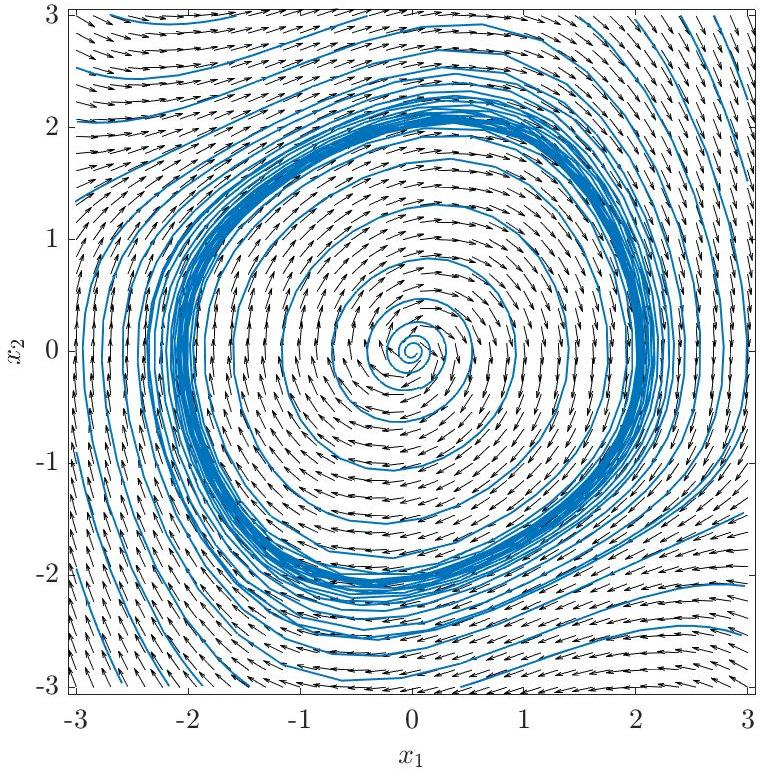
\includegraphics[width = 0.4\textwidth]{figures/system2.jpg}
    \caption{A Van der Pol system $\dot x + 0.2(x^2-1)\dot x + x = 0$}
    \label{fig:van-der-pol}
\end{figure}

The state space form for the simple harmonic oscillator state vectors is $x_1 = x , x_2=\dot x$, for $\dot x_1 = x_2$ and $\dot x_2 = -kx_1$. The state space form for the Van der Pol system is $x_1 = x$, $x_2 = \dot x$, for $\dot x_1 = x_2$ and $\dot x_2 = 0.2(1-x_1^2)x_2-x_1$.

The key differences between a simple sustained oscillation (such as in our first system) and limit cycle (such as in our second system) are twofold. First, the amplitude of a limit cycle is independent of its initial conditions. Once the limit cycle is reached, irregardless of where it started, it will continue through the self-sustaining limit cycle loop. In a simple oscillation, initial conditions are what determines which of the oscillations it can reached.

The second difference is that simple oscillations are extremely sensitive to system parameter changes. A small change can either cause the system to converge or become unstable. A limit cycle, however, is less susceptible to initial conditions heavily affecting the behaviour of the system.

\section*{Problem 2}

In this problem, we are presented with a pendulum system defined by the equation $ml^2\ddot{q}=mgl\sin{q}+u$.

\subsection*{Part A}

Here, we let:

\[x = \begin{bmatrix} x_1 \\ x_2 \end{bmatrix} = \begin{bmatrix} q \\ \dot{q} \end{bmatrix}\]

We then find the state space formulation of the system (assuming $u(t)=0$) by definining $\dot{x}_1$ and $\dot{x}_2$:

\[\begin{bmatrix}\dot{x}_1\\\dot{x}_2\end{bmatrix}=\begin{bmatrix}x_2\\ \frac{mgl\sin{x_1}}{ml^2}\end{bmatrix}=\begin{bmatrix}
x_2 \\ gl^{-1}\sin{x_1}
\end{bmatrix}\].

\subsection*{Part B}

Assuming the $m=0.1$ kg , $l=1$ m, and $g=9.81$ $\frac{m}{s^2}$, we utilize MATLAB to draw a phsae portrait of the system provided. We make use of provided ranges, $-3\pi \leq x_1 \leq 3\pi$ and $-4 \leq x_2 \leq 4$. The phase portrait generated is below:

\begin{figure}[H]
    \centering
    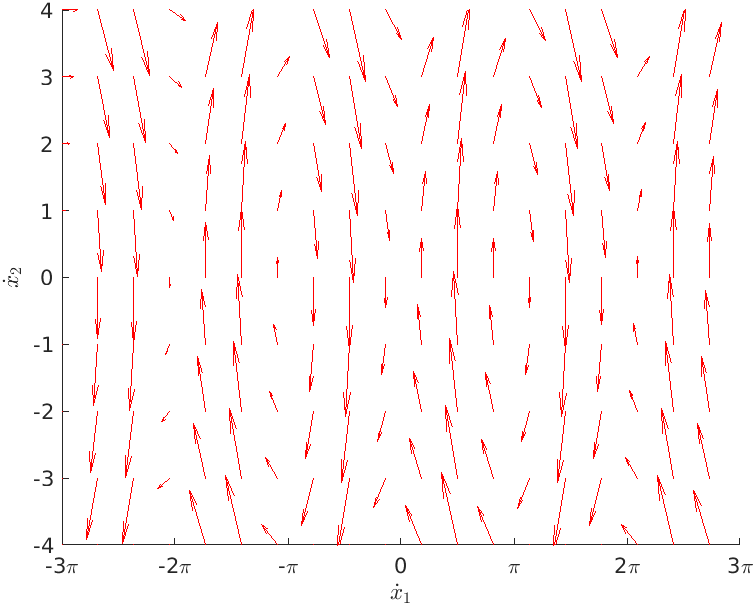
\includegraphics[width = 0.4\textwidth]{figures/phase_portrait.png}
    \caption{Phase portrait of our system pendulum system}
    \label{fig:phase-portrait}
\end{figure}

The portrait is created via the MATLAB code listed in the code subsection.

\subsection*{Part C}

In this problem, we are tasked to utilize the phase portrait from Part B and identify the equilibrium points of the system, classifying them into stable or unstable groups.

Using the phase portrait from before, we solved the ordinary differential equation for different initial conditions to better demonstrate the system's diverging and converging behaviours. We then highlighted key points that we believe are equilibrium points.

\begin{figure}[H]
    \centering
    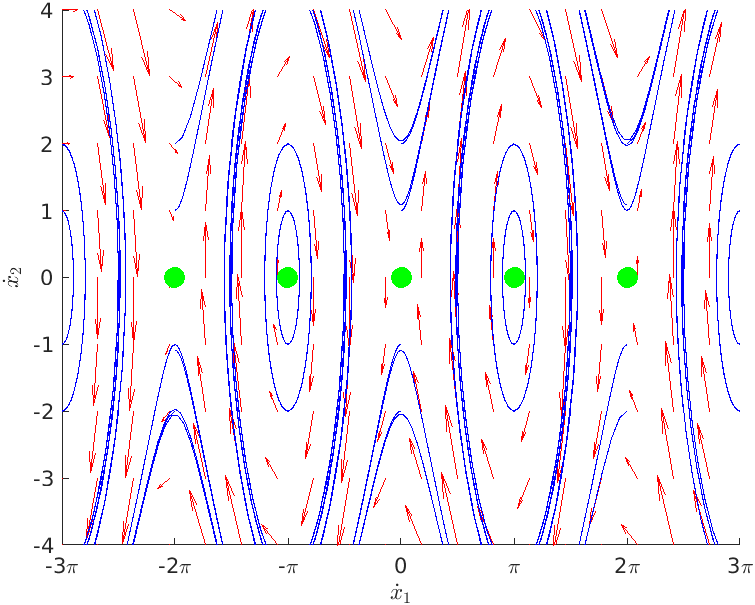
\includegraphics[width = 0.4\textwidth]{figures/phase_portrait_with_equilibrium_points.png}
    \caption{Phase portrait of our pendulum system with equilibrium points}
    \label{fig:phase-portrait-equilibrium}
\end{figure}

The above figure was created via MATLAB code found in the Code subsection.

When $\dot{x}_2 = 0$, we have an equilibrium point. When the equilibrium point is an odd integer multiple of $\pi$ - ie $-\pi$ or $\pi$ - the system acts as if it converges towards the equilibrium point and is thus \textbf{stable}. Note that it never actually converges onto these points in this system - these are defined as \textit{center points}. At even integer multiples of $\pi$ - ie $-2\pi$ or $2\pi$ - the system diverges away from the equilibrium point, and is thus \textbf{unstable}.

This makes sense when considering that the system proposed is a pendulum. Imagine a pendulum held above it's rotation point, perfectly vertical. This is the even $\pi$ rotational positions. The pendulum would remain in this position absent any additional disturbances or outside forces. Small forces add to this system would cause it to immediately diverge from this position, however. Alternatively, on odd $\pi$ rotational positions, the pendulum is at the bottom of its rotation. Any small changes likely cause it to return back to its resting position straight down.

\subsection*{Code}

\subsubsection*{Phase Portrait Code}
This code was utilized to create Figure \ref{fig:phase-portrait}.

\begin{center}
    \begin{lstlisting}[caption={Phase Portrait MATLAB code},captionpos=b, language=MATLAB]
        figure
        hold on
        xlabel('$\dot{x}_1$','interpreter','latex');
        ylabel('$\dot{x}_2$','interpreter','latex');
        xlim([-3*pi 3*pi]);
        ylim([-4 4]);
        set(gca,'XTick',-3*pi:pi:3*pi);
        set(gca, 'XTickLabel',{'-3\pi','-2\pi','-\pi','0','\pi','2\pi','3\pi'});
        
        m = 0.1;
        l = 1;
        g = 9.81;
        
        [x1,x2] = meshgrid(-3*pi:3*pi,-4:4);
        
        dx1 = x2;
        dx2 = (m*g*l*sin(x1))/(m*l^2);
        quiver(x1, x2, dx1, dx2, 'color', 'red')
        hold off
    \end{lstlisting}
\end{center}

\subsubsection*{Phase Portrait with Equilibrium Points Code}
This code was utilized to create Figure \ref{fig:phase-portrait-equilibrium}.

\begin{center}
    \begin{lstlisting}[caption={Phase Portrait with Equilibriums MATLAB code},captionpos=b, language=MATLAB]
        figure
        hold on
        xlabel('$\dot{x}_1$','interpreter','latex');
        ylabel('$\dot{x}_2$','interpreter','latex');
        xlim([-3*pi 3*pi]);
        ylim([-4 4]);
        set(gca,'XTick',-3*pi:pi:3*pi);
        set(gca, 'XTickLabel',{'-3\pi','-2\pi','-\pi','0','\pi','2\pi','3\pi'});

        quiver(x1, x2, dx1, dx2, 'color', 'red')

        f = @(t, X) [X(2); (m*g*l*sin(X(1)))/(m*l^2);];

        for x1_initial = -3*pi:pi/2:3*pi
            for x2_initial = -2:1:2
                [ts, q] = ode45(f, [0, 4],[x1_initial, x2_initial]);
                
                % Plot our line for the given initial conditions
                plot(q(:,1), q(:,2), 'Color', 'blue');
            end
        end

        equilibrium_points = [0 0; -pi 0; -2*pi 0;pi 0; 2*pi 0;];

        plot(equilibrium_points(:,1), equilibrium_points(:,2), 'LineStyle',"none", 'Marker',"o", 'MarkerSize', 10, 'MarkerEdgeColor', "green", 'MarkerFaceColor', 'green')

        hold off
    \end{lstlisting}
\end{center}

\end{document}
